\documentclass[12pt]{article}

\usepackage[total={6.5in,8.75in}, top=2.4cm, left=2.4cm]{geometry}
\usepackage{lineno}
\usepackage{amsmath}
%\usepackage{amssymb}    % used for symbols in figure legends
\usepackage{graphicx}
\usepackage[round,colon,authoryear]{natbib}

\usepackage{bm}
\usepackage{float}
\usepackage{amsmath}
\usepackage{amsfonts}
\usepackage{hyperref}
\usepackage{verbatim}
\usepackage{soul}
\usepackage{color}
\usepackage{setspace}

\bibliographystyle{ecology} % kluwer, plos-natbib, pnas-natbib


\title{Integrating
Resource Selection Information with Spatial Capture-Recapture}

\begin{small}
\author{
{\bf J. Andrew Royle} and {\bf Richard B. Chandler}
\\
USGS Patuxent Wildlife Research Center, Laurel MD \\ \\
}
\end{small}


\begin{document}

\maketitle

\date


\linenumbers


\begin{spacing}{1.2}

\begin{flushleft}
{\em \bf Abstract.}
%Two of the most important objectives in studies of animal populations
%are the estimation of resource selection and population size
Understanding space usage and resource selection is a primary focus of
many studies of animal populations. Usually, such studies are based on
location data obtained from telemetry,
%used to record movements or dispersal events
and resource selection functions (RSF) are used for inference.
Another important focus of wildlife research is estimation and
modeling population size and density.
%On the other hand,
Spatial capture-recapture (SCR) models accomplish this objective
%provide a framework for estimating density of animal populations
using individual encounter history data with auxiliary spatial information
on location of capture. Although the encounter probability models used in SCR
are intuitively related to space usage, to date, no one has extended
SCR models to allow for explicit inference about
%methods of using SCR data to study
space usage and resource selection. % have been proposed.
In this paper we develop the first statistical framework for
jointly modeling space usage, resource selection, and population
density by integrating SCR data, such as from camera traps, mist nets, or
conventional catch-traps, with resource selection data from telemetered individuals.
We provide a framework for estimation based on marginal
likelihood, wherein we estimate simultaneously the parameters of the
SCR model and RSF model.  Our method leads to increases in precision
for estimating animal abundance or density, and parameters of ordinary
SCR models.  Importantly, we also find that SCR models {\it alone} can
estimate parameters of resource selection functions and, as such, SCR
methods can be used as the sole source for studying space-usage;
%in place of conventional animal telemetry.
however, precision will be higher when telemetry data are available.
Finally, we find that SCR
models using standard symmetric and stationary encounter probability
models produce biased estimates of density when animal space
usage is related to a landscape covariate. Therefore, it is
critically important that space usage be taken into consideration, if
possible, in studies focused on estimating density using
capture-recapture methods.

{\em \bf Key words:} animal movement, animal sampling, encounter
probability, hierarchical modeling, landscape connectivity, marginal likelihood,
resource selection, space usage,  spatial capture-recapture.

\end{flushleft}



\chapter{
Modeling Space Usage:
Integrating Resource Selection Information with
Spatial Capture-Recapture
  Models}

\markboth{Resource Selection and Space Usage}{}
\label{chapt.rsf}


\vspace{.3in}

Up to this point we have developed many variations of
SCR models to describe the observation process. 
These included models of the relationship between encounter
probability and distance, and different types of covariates such as 
behavioral responses 
that can affect detection
probability. 
Although these different observation models are immensely useful, they
are rather basic in the sense
that they imply simplistic models of how individuals use space
(section \ref{scr0.sec.implied}) and how individuals are distributed
in space.  In the following several chapters we generalize some of the
core SCR assumptions to accommodate more realistic notions of how
animals use space.

In this chapter we extend our notion of encounter probability models
as models of space usage or resource selection
(sec. \ref{scr0.sec.implied}), by extending them to include one or
more explicit landscape covariates, which the investigator believes
might affect how individual animals use space within their home range
(this is what \citep{johnson:1980} called {\it third-order} selection). We do this in a way
that is entirely consistent with the manner in which classical
``resource selection function'' (RSF) models \citep{manly_etal:2002} or utilization
distributions \citep{worton:1989, fieberg:2005, fieberg:2007}are estimated from animal
telemetry data.  In fact, we argue there that SCR models and RSF/UD
models estimated from telemetry are based on the same basic underlying model
of space usage. The important distinction between SCR and RSF studies are
that, in SCR studies, encounter of individuals is imperfect (i.e.,
``$p<1$'') whereas, with RSF data obtained by telemetry, encounter is
perfect\footnote{this is not strictly true -- rather, detection is not
  a {\it stochastic} outcome.}. We can think of the two as being
exactly equivalent either if we have a dense array of trapping
devices, or if our telemetry apparatus is imperfect such as only
samples a small area of space (this would be consistent with telemetry
stations for sampling fish which only measure passage).  A key concept
that we must confront in order to unify and integrate SCR and RSF data
is that we need to formulate both models in terms of a common latent
variable so that we can make them consistent with respect to some
underlying space utilization process. As we will explain, this latent
variable is the number of times that an individual uses a 
particular pixel of the landscape.

Here we show how to integrate standard RSF type data obtained from
telemetry into SCR models to model space usage explicitly.  This
produces asymmetric, irregular and non-stationary home ranges, and
allows us to make formal inferences about factors that influence home
range geometry and morphology directly from SCR data.  We begin by
describing a model for space usage that exists independent of how we
obtain the data (whether by telemetry or by capture-recapture). The
model posits that individuals use space in proportion to one or more
measurable covariates, say $z({\bf x})$, defined for every pixel or
location ${\bf x}$.  Then we introduce observation models consistent
with both standard capture-recapture methods and telemetry.  This
allows us to define a general likelihood function that is the product
of the two components, if they are both simultaneously available.  In
the absence of RSF data from telemetry, the model reduces to an
ordinary SCR model but with a spatial covariate $z({\bf x})$ affecting
encounter probability.

Following \citet{borchers_efford:2008}, we provide a formal
likelihood-based analysis of the model, and carry-out a simulation
study for various sample sizes of telemetered individuals to evaluate
the improvement from adding telmetry information to SCR studies and
{\it vice versa}.
The modeling framework we develop here simultaneously resolves
 three important
technical problems: (1) it generalizes all existing
encounter probability models for SCR data to accommodate realistic
patterns of space usage that are {\it not} symmetric and spatially
constant;
(2) It allows us to estimate RSF
parameters directly from SCR data, i.e., {\it absent} telemetry data;
and (3) it allows us to integrate telemetry data directly into SCR
models to improve estimates of model parameters, including density.
Our model greatly expands the applied relevance of SCR methods for
conservation and management, and for addressing applied and theoretical
questions related to animal space usage.


\begin{comment}
In our formulation we estimate the latent ${\bf s}$ variables from the observed telemetry
data, just as a convenience, but this wouldn't be necessary.
Also we assume the data are independent pieces but if some of the SCR
individuals are the same as the telemetered individuals then we should
probably account for that explicitly. So right now we pretend we don't
know anything about the telemetered guys in terms of their capture
history. So they don't contribute to information about baseline
encounter probability, just to estimates of the other encounter model
parameters.
\end{comment}



\section{Basic Model of Space Usage}
\label{rsf.sec.rsfmodel}

We develop the model here in terms of a discrete landscape purely for
computational expediency. That said, essentially no landscape on your
computer is continuous, except in the rare case that the landscape is
defined strictly in terms of variables that themselves are inherently
continuous -- e.g., ``distance to road'' or something like that.  But
almost all habitat or landscape structure data comes to us in the form
of raster data.  Let ${\bf x}_{1},\ldots,{\bf x}_{nG}$ identify the center
coordinates of a set of $nG$ pixels that define a landscape.
We organize them into a matrix
${\bf X}_{nG \times 2}$.  Let $z({\bf x})$ denote a covariate measured
(or defined) for
every pixel ${\bf x}$. For clarity, we develop the basic ideas here in terms of a
single covariate but, in practice, investigators typically have more
than 1 covariate. The formulation of the model is unaffected by
whether we have one or multiple such covariates.

We suppose that a population of individuals wanders around space in
some manner related to the covariate $z({\bf x})$, and their locations
accumulate in pixels by some omnipotent accounting mechanism. We will
define ``use of ${\bf x}$'' to be the event that an individual animal
appeared in some pixel ${\bf x}$. This is equivalently stated in the
literature in terms of individual having {\it selected} ${\bf x}$ but
the latter term implies some kind of 
conscious intent, and so we keep to the term {\it use} as much as
possible.
As a biological matter, use is the outcome of
individuals moving around their home range but, i.e., where an
individual is at any point in time is the result of some movement
process. But, to understand space usage, it is not necessary to
entertain explicit models of movement, just to observe the outcomes,
and so we don't elaborate further on what could be sensible or useful
models of movement.

Let $n_{ij}$ be the number of times individual $i$ used pixel $j$
during some period of time, i.e., the use frequencies.  We assume the
following probability mass function for the distribution of use
frequencies:
\[
{\bf n}_{i} \sim \mbox{Multinom}({\bm \pi}_{i})
\]
where
\[
 \pi_{ij} = \frac{ exp( \alpha_{2} z({\bf x}) ) }{ \sum_{x}
   exp(\alpha_{2} z({\bf x}))}
\]
This is the standard RSF model \citep{manly_etal:2002} used to model
telemetry data.  The parameter $\alpha_2$ is the effect of the
landscape covariate $z({\bf x})$ on the relative probability of
use. Thus, if $\alpha_2$ is positive, the relative probability of use
decreases as the covariate increases. In practice, we don't get to
observe $n_{ij}$ for all individuals but, instead, only for a small
subset which we capture and install telemetry devices on.  For these
telemetered individuals we accumulate individual- and pixel-specific
frequencies, at a lower sampling rate than actual individual use. For
example, we might choose to record the location of an individual every
hour or day or whatever. As such, the observed frequency of pixel use
is a {\it sample} of use but, if the recording is random or systematic
(or otherwise unrelated to {\it where} individuals are located), then
we can imagine that the same model of space usage applies. Formally,
we suppose that the observed frequencies are a binomial sample with
sample size $n_{ij}$ and sampling intensity $\phi_{0}$ lets say, and
we see that the constant $\phi_{0}$ cancels from the expression for
the multinomial cell probabilities above. 
Therefore, for the
telemetered individuals, we adopt the standard RSF model which has
probabilities as above:
\[
 \pi_{ij} = \frac{ exp( \alpha_{2} z({\bf x}_{j}) ) }{ \sum_{x}   exp(\alpha_{2} z({\bf x}_{j}))}
\]
We extend this model slightly to make it more realistic spatially. Let
${\bf s}$ denote the centroid of an individuals home range and let
$D_{ij} = ||{\bf x}_{j} - {\bf s}_{i}||$ be the distance from the home
range center of individual $i$, ${\bf s}_{i}$, to pixel $j$, ${\bf
  x}_{j}$. We modify the space usage model to accommodate that space
use will be concentrated around an individuals home range centroid:
\begin{equation}
 \pi_{ij} = \frac{ exp( -\alpha_{1} D_{ij}^{2} +\alpha_{2} z({\bf x}_{j}) ) }
{ \sum_{x} exp(-\alpha_{1} D_{ij}^{2} +\alpha_{2} z({\bf x}_{j}))}
\label{rsf.eq.rsf}
\end{equation}
where $\alpha_1=1/(2\sigma^2)$ describes the rate at which capture probability
declines as a function of distance. Note that Eq.~\ref{rsf.eq.rsf} resembles standard encounter models
used in spatial capture-recapture but with an additional covariate
$z({\bf x})$ (and see Chapt. \ref{chapt.poisson-mn}).
In particular, under this model for space usage or resource selection,
if you have no covariates at all, or if $\alpha_{2} =
0$, then
the probabilities $\pi_{ij}$ are directly proportional to the SCR
model for encounter probability.
For example, setting $\alpha_{2} = 0$, then this implies probability
of use for pixel $j$ is:
\[
p_{ij} \propto  exp( -\alpha_{1} D_{ij}^{2})
\]
so whatever function of distance we use in our RSF implies an
equivalent model of space usage (sec. \ref{scr0.sec.implied})
when used in SCR models. Another difference between this observation model
and those that we have considered previously is that it includes a
normalizing constant $\sum_{x} exp(-\alpha_{1} D_{ij}^{2} +\alpha_{2}
z({\bf x}_{j}))$, which ensures that the use distribution is a 
proper probability density function. Thus we are able to compute
the relative probability of capture in terms of distance and space use.

As an illustration of space usage patterns under this model, we
simulated a covariate that represents 
variation in habitat
structure (Fig. \ref{rsf.fig.habitat}) such as might correspond to
habitat quality.
\begin{figure}
\centering
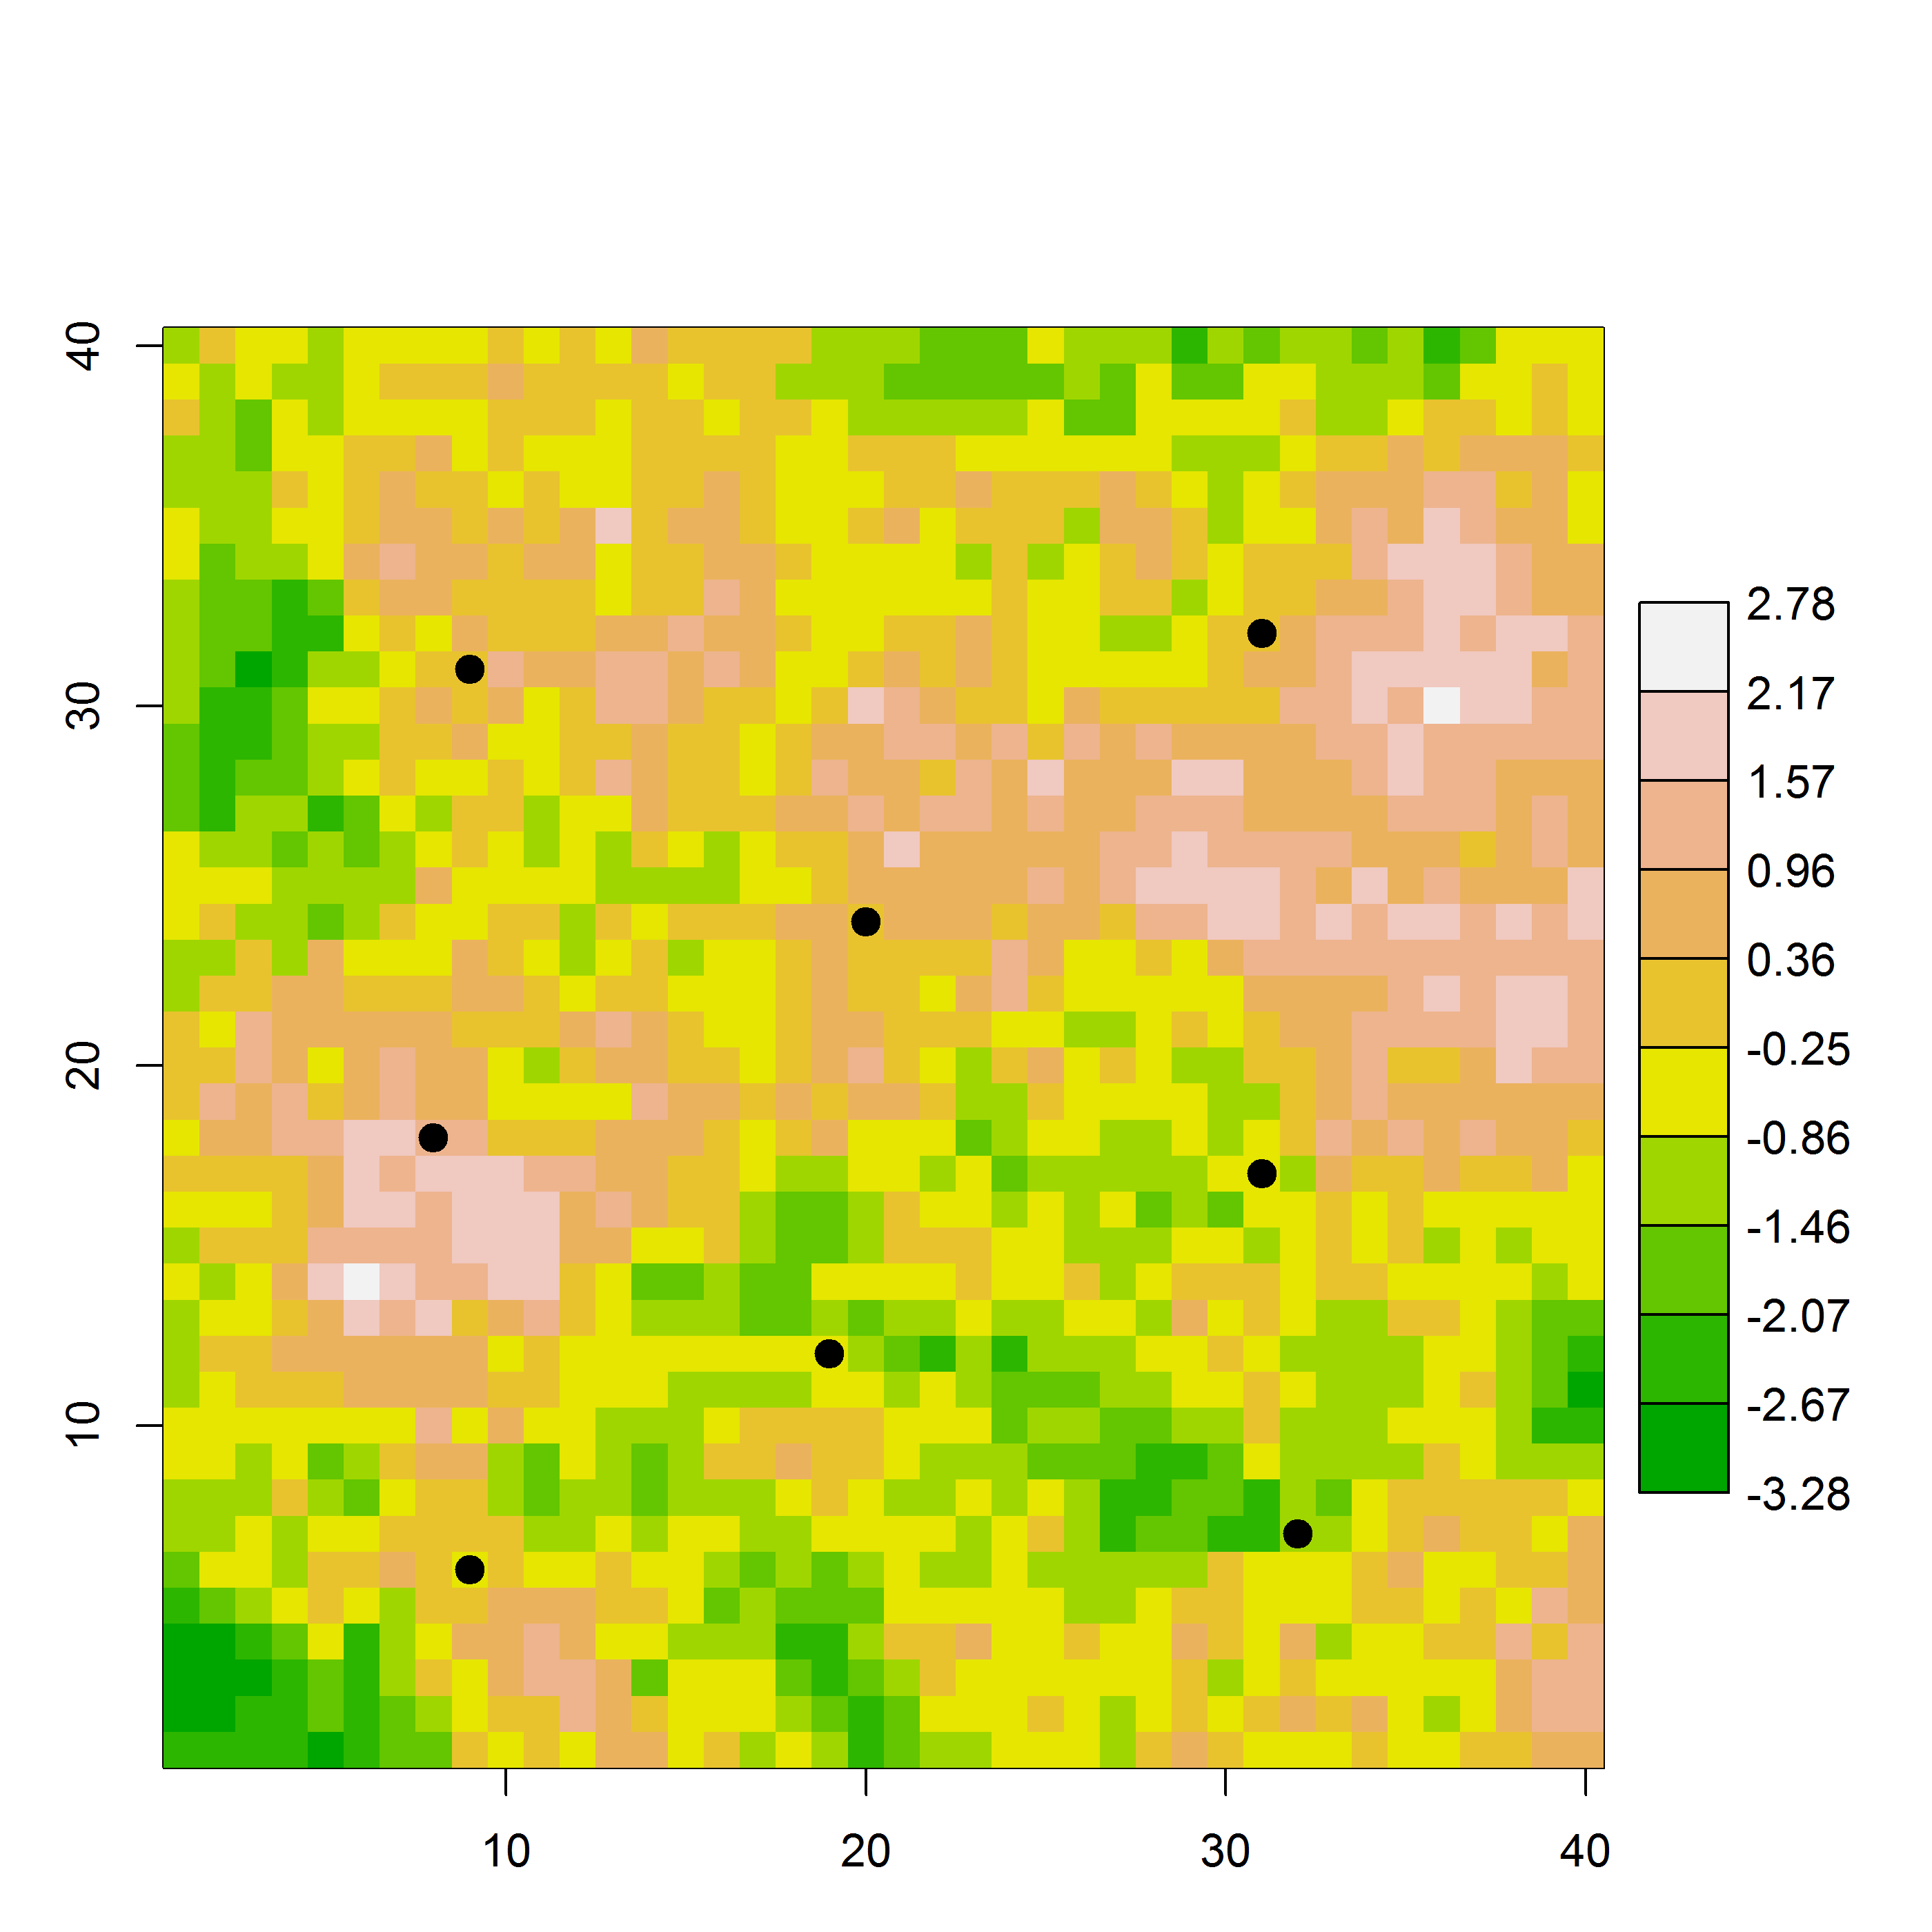
\includegraphics[width=3.5in,height=3.5in]{Ch10b/figs/habitat}
\caption{A typical habitat covariate reflecting habitat quality or
  hypothetical utility of the landscape to a species under study. Home range centers for 8 individuals are
shown with black dots.}
\label{rsf.fig.habitat}
\end{figure}
This was simulated by using a
kriging interpolator with the following {\bf R} commands:
\begin{verbatim}
set.seed(1234)
gr<-make.statespace(minx=1,maxx=40,miny=1,maxy=40,nx=40,ny=40)
Dmat<-as.matrix(dist(gr))
V<-exp(-Dmat/5)
z<-t(chol(V))%*%rnorm(1600)
spatial.plot(gr,z)
\end{verbatim}
The functions \mbox{\tt make.statespace} and \mbox{\tt spatial.plot} are
both in the \mbox{\tt scrbook} package.
Space usage patterns for
 8 individuals are shown in Fig. \ref{rsf.fig.homeranges},
simulated with $\alpha_{1} = 1/(2\sigma^2)$ with $\sigma = 2$ and the
coefficient on $z({\bf x})$ set to $\alpha_{2} = 1$.
\begin{figure}
\centering
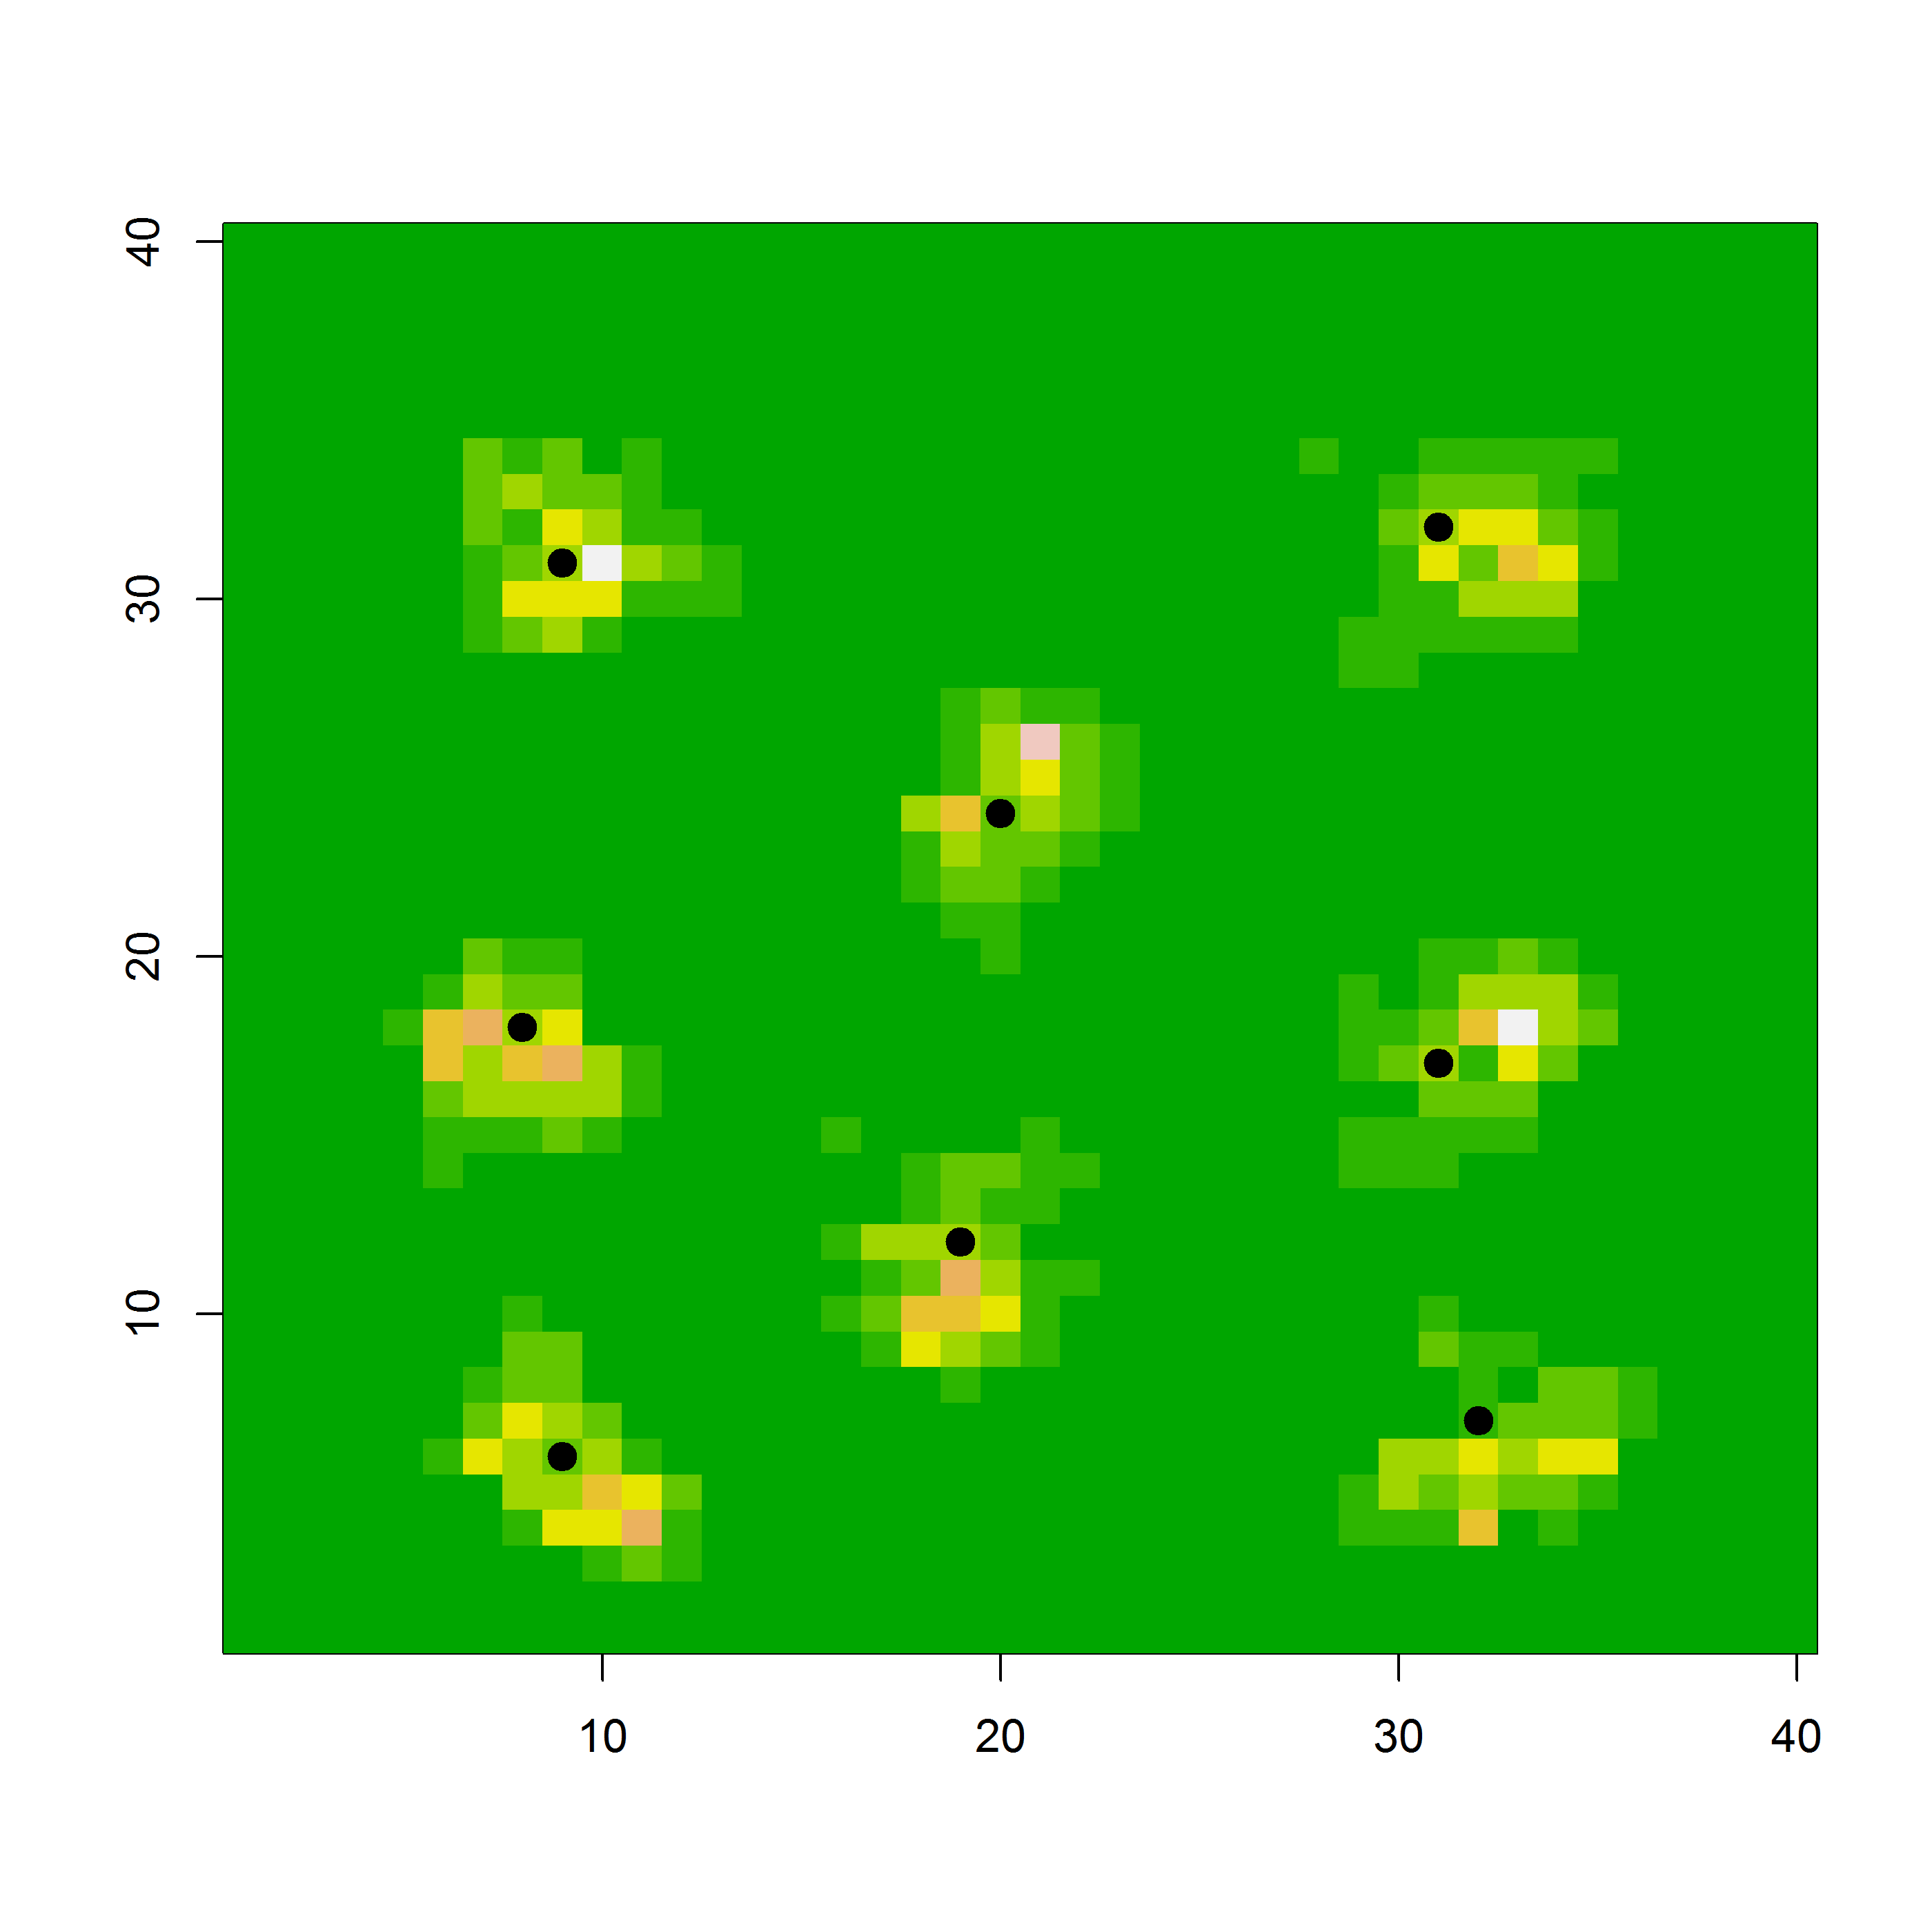
\includegraphics[width=3.5in,height=3.5in]{Ch10b/figs/homeranges8}
\caption{Space usage patterns of 8 individuals under a space usage
  model that contains a single covariate (shown in
  Fig. \ref{rsf.fig.habitat}). Plotted value is the multinomial
  probability $\pi_{ij}$ for pixel $j$ under the model in Eq. \ref{rsf.eq.rsf}.
}
\label{rsf.fig.homeranges}
\end{figure}
These space usage densities -- ``home ranges'' -- exhibit clear
non-stationarity in response to the structure of the underlying
covariate, and they are distinctly asymmetrical.  We note that if
$\alpha_{2}$ were set to 0, the 8 home ranges shown here would
resemble bivariate normal kernels with $\sigma = 2$.  Another
interesting thing to note is that the activity centers are not
typically located in the pixel of highest use or even the centroid of
usage. That is, the observed ``average'' location is not an
unbiased estimator of ${\bf s}$ under the model in
Eq. \ref{rsf.eq.rsf}. 



\subsection{Poisson use model}

A natural way to motivate this specific model of space usage is to
assume that individuals make a sequence of random resource selection
decisions so that the outcome of $n_{ij}$ are marginally {\it
  independent}, having a Poisson distribution:
\[
 n_{ij} \sim \mbox{Poisson}( \lambda_{ij})
\]
where
\[
 log(\lambda_{ij}) = a_{0} -\alpha_{1} D_{ij}^{2} +  \alpha_{2} z({\bf x})
\]
In this case,
 the number of visits to any particular cell is affected by
the covariate $z({\bf x})$ but has a baseline rate ($exp(a_{0})$) related to the amount
of movement, or number of selection decisions which is essentially
just related to the time interval over which the animal is using
space. i.e., longer time intervals lead to higher values of
$E(n_{ij})$.
This is an equivalent model to the multinomial model given previously
in the sense that, if we condition on the total sample size $n_{i.} =
\sum_{j} n_{ij}$, then the vector ${\bf n}_{i}$ has a multinomial
distribution with probabilities
\[
 \pi_{ij} = \frac{\lambda_{ij}}{ \sum_{j} \lambda_{ij}}
\]
as we discussed in Chapt. \ref{chapt.poisson-mn}.  We see that the
intensity parameter $a_{0}$ is not relevant for understanding
patterns of space usage. In particular, it cancels from the numerator
and denominator of the multinomial cell probabilities, analogous to
what happens under sampling of individual use decisions as discussed
above.

\begin{comment}
{\bf note:} while Poisson -> multinomial, it is not vice versa. If the total
sample size per individual is fixed, then the marginals are NOT
Poisson and that model will produce biased estimators.

For purposes of estimation we can use either the Poisson or
multinomial likelihoods. In the former case, we have to estimate an
individual-specific nuisance
parameter $a_{0}$, from which information is derived by the total
number of observations whereas, in the later case, we lose information
about $a_{0}$ by conditioning on the total (i.e., treating it as
fixed).  As it often is fixed, or at least the number of telemetry
observations is completely arbitrary, $a_{0}$ is usually a meaningless
parameter so whether we estimate it or not is immaterial from a
practical standpoint.
\end{comment}

\subsection{Thinning}

Suppose our sampling is imperfect so that we only observe a smaller
number of telemetry fixes than actual uses, $n_{ij}$. As developed in
sec. \ref{scr0.sec.implied}, we assume that the observed number of
uses is
\[
 m_{ij} \sim \mbox{Bin}(n_{ij}, \phi_{0}).
\]
In this case, the marginal distribution of $m_{ij}$ is also Poisson
but with mean
\[
 log(\lambda_{ij}) = log(\phi_{0}) + a_{0} -\alpha_{1} D_{ij}^{2} +  \alpha_{2} z({\bf x}).
\]
In this case, the space-usage model (RSF) for the
thinned counts $m_{ij}$ is the same as the space-usage model for the
original variables $n_{ij}$.  This is because if we remove $n_{ij}$
from the conditional
 model by summing over its possible values, then the vector of
${\bf m}_{i}$ is multinomial with cell probabilities
\[
\frac{\phi_{0}\lambda_{ij}}{\sum_{j} \phi_{0} \lambda_{ij}}
\]
and we see that $\phi_{0}$ cancels from the numerator and
denominator. XXXX not really elucidating here XXXXXXX

%That is,
%given our sequence of
%independent Poisson random variables and we condition on their total,
%i.e., regard it as fixed, then we have the multinomial. In the
%multinomial we lose information about the intercept which in this case
%is ok because we only care about the interpretation of the resource
%selection model as a probability distribution and don't care about the
%basic rate of detection -- and it is a confounding of animal use and a
%fixed sampling intensity.

In summary, if we conduct a telemetry study we observe ${\bf n}_{i}$,
the $nG \times 1$ vector of pixel-counts for each individual
$i=1,\ldots,N_{tel}$.  We declare these data to be
``resource-selection data'' which are typical of the type used to
estimate resource-selection functions (RSFs) \citep{manly_etal:2002}.
Sometimes in RSF modeling activities people make believe they have
continuous covariates and so the denominator in Eq. \ref{rsf.eq.rsf}
involves an integration over a distribution for the covariate which is
the conditional intensity of observed point locations in a point
process model. However, in a discrete landscape, entertaining pdfs for
the covariates isn't necessary \citep{royle_etal:2012mee}.\hl{Or is it
  that they ignore the fact that they are sampling 2D space? They seem
  to act as if they are sampling K-dimensional covariate space.}
\hl{yea, this could be it. lets contemplate this}

\subsection{Capture-recapture Data}

The key to combing RSF data with SCR data is to work with this
underlying resource utilization process and formulate SCR models in
terms of that process. For SCR models, the frequency of use for each pixel
serves as a intermediate
latent that we don't get to observe. We assume that, fundamentally,
both telemetered individuals and SCR individuals are using space
according to the same resource selection model. The difference is that,
for SCR data, we 
do not have sampling devices in all locations (pixels) in the landscape, and hence the
data are only recorded at a subsample of them.
In other words, imagine that we have a sampling device, such as a
camera trap, in {\it every} pixel. If the device operates continually
then it is no different from a telemetry instrument. If it
operates  intermittently and does not expose the entire area of
each pixel then a reasonable model for this imperfect observation is
the ``thinned'' binomial model given above, where $\lambda_{0}$
represents the sampling effectiveness of the device. So we imagine
that the hypothetical perfect data from a camera trapping study are
the counts $m_{ij}$.

We then construct our SCR encounter probability model based on the
view that these frequencies $m_{ij}$ are {\it latent}. In particular,
under the SCR model with binary observations,
 we observe a random variable
$y_{ij} = 1$  if the individual $i$ visited the pixel
containing a trap and was detected.
We imagine that $y_{ij}$ is related to the latent variable $m_{ij}$ being the
event $m_{ij}>0$, which occurs with probability
\[
 p_{ij} = 1-exp(- \lambda_{ij})
\]
where 
\[
 log(\lambda_{ij}) = log(\phi_{0}) + a_{0} -\alpha_{1} D_{ij}^{2} +  \alpha_{2} z({\bf x}).
\]
and we collect the constants so that $\alpha_{0} = log(\phi_{0}) +
a_{0}$ is the 
 baseline encounter rate which includes
the constant intensity of use by the individual and also the baseline
rate of detection, conditional on use.



\section{The Joint RSF/SCR Likelihood}

To construct the likelihood for SCR data when we have auxiliary
covariates on space usage {\it or} direct information on space usage
from telemetry data, we regard the two samples (SCR and RSF) as
independent of one another. In practice, this might not always be the
case but (1) often time the telemetry data come from a previous study;
(2) the individuals are not the same at all; (3) or even if they are
some of the same individuals being captured, we might not be able to
match individuals captured by a sampling method such as hair-snares
with the individuals wearing radio-collars; (4) In cases where we {\it
  can} match some individuals between the two samples, regarding them as
independent should only entail a minor
loss of efficiency
because we are disregarding more precise information on a small number
of activity centers. Moreover, we believe, it is unlikely in practice
to expect the two samples to be completely reconcilable and that the
independence formulation is the most generally realistic.

Regarding the two data sets as being independent, our approach here
is to form the likelihood for each set of observations as a function
of the same underlying parameters and then combine them. In
particular, let ${\cal L}_{scr}(\alpha_{0}, \alpha_{1}, \alpha_{2}, N;
{\bf y}_{scr})$
be the likelihood for the SCR data in terms of the basic encounter
probability parameters and the total (unknown) population size $N$,
and let ${\cal L}_{rsf}(\alpha_{1},\alpha_{2}; {\bf m}_{rsf})$ be the
likelihood for the RSF data based on telemetry which, because the
sample size of such individuals is fixed, does not depend on $N$.
The
joint likelihood is the product of these two pieces:
\[
{\cal L}_{rsf+scr}(\alpha_{0},\alpha_{1},\alpha_{2},N; {\bf y}_{scr},{\bf
  m}_{rsf})  = {\cal L}_{scr} \times {\cal L}_{rsf}
\]
In what follows, we provide a formulation of each likelihood
component, along with an {\bf R} function for obtaining the MLEs of
model parameters using standard methods available in {\bf R}.

The observation model for the SCR data for individual $i$ and trap $j$,
from sampling over $K$ encounter periods, is:
\[
 y_{ij}|{\bf s}_{i} \sim \mbox{Bin}(K; p_{ij})
\]
where
\[
 p_{ij} = 1-exp(- \lambda_{ij} )
\]
and
\[
 \lambda_{ij} = \lambda_{0} exp(- \alpha_{1} D_{ij}^{2} + \alpha_{2}  z(x_{j}) )
\]
A compact expression of these model components is:
\begin{equation}
y_{ij}| {\bf s}_{i} \sim \mbox{Bin}(K, p_{\alpha}(D_{ij}; {\bm \alpha}))
\label{rsf.mle.eq.cond-on-s}
\end{equation}
We emphasize that this is conditional on the latent variables ${\bf
  s}_{i}$ (which appear in $D_{ij}$). For these latent variables we
adopt the standard assumption of uniformity, ${\bf s}_{i} \sim
\mbox{Unif}({\cal S})$.  The joint distribution of the data for
individual $i$, conditional on ${\bf s}_{i}$, is the product of $J$
binomial terms (i.e., the contributions from each of $J$ traps):
\[
  [{\bf y}_{i} | {\bf s}_{i} , {\bm \alpha}] =
  \prod_{j=1}^{J} \mbox{Bin}(K, p_{\alpha}({\bf x}_{j},{\bf s}_{i}) )
\]
The so-called marginal likelihood \citep{borchers_efford:2008} is
computed by removing ${\bf s}_{i}$, by integration, from the
conditional-on-${\bf s}$ likelihood and regarding the {\it marginal}
distribution of the data as the likelihood. That is, we compute:
\[
  [{\bf y}_{i}|{\bm \alpha}] =
\int_{{\cal S}}  [ {\bf y}_{i} |{\bf s}_{i},{\bm \alpha}] g({\bf s}_{i}) d{\bf s}_{i}
\]
{\flushleft where}, under the uniformity assumption, we have
$g({\bf s}) = 1/||{\cal S}||$.
The joint likelihood for all $N$ individuals,
is the product of $N$ such terms:
\[
{\cal L}_{scr}({\bm \alpha} | {\bf y}_{1},{\bf y}_{2},\ldots, {\bf y}_{N}) = \prod_{i=1}^{N}
[{\bf y}_{i}|{\bm \alpha}]
\]
Now, in practice, we don't know $N$ and so we can't just compute the
SCR likelihood in this manner. Following our development in
Chapt. \ref{chapt.mle},
we can compute the contributions of the
$n$ observed individuals, but then we have to compute the likelihood
contribution for the ``all 0'' encounter history, i.e., that
corresponding to unobserved individuals. The mechanics of computing
that are the same as for an ordinary observed encounter history. We
then have to deal with the issue that $n$ itself is a random variable,
and that leads to the combinatorial term in front of the likelihood
which involves the total population size $N$.

For the RSF data from the sample of individuals with telemetry devices
we adopt the same basic strategy of describing the
conditional-on-${\bf s}$ likelihood and then computing the marginal
likelihood by averaging over possible values of ${\bf s}$.
We have ${\bf m}_{i}$, the vector of pixel counts for individual $i$,
where these counts are derived from a telemetry study or similar.
Their likelihood contribution is
proportional to
\[
 {\cal L}_{rsf}({\bm \alpha}, {\bf m}_{rsf})
 = \prod_{g=1}^{G}  \pi_{ij} ^{m_{ij}}
\]
where
\[
 \pi_{ij} =  = \frac{ exp( -\alpha_{1} D_{ij}^{2} -\alpha_{2} z({\bf x}_{j}) ) }
{ \sum_{g} exp(-\alpha_{1} D_{ij}^{2} -\alpha_{2} z({\bf x}_{j}))}
\]

Technical details for computing the likelihood and obtaining the MLEs
are given in Appendix 1 where we provide an ${\bf R}$ function to
evaluate the likelihood and obtain the MLEs.
\begin{comment}
\begin{verbatim}

Script here

\end{verbatim}
\end{comment}
A key practical detail
is that the likelihood here is formulated in terms of the parameter
$N$, the population size for the landscape defined by ${\cal
  S}$. Given ${\cal S}$, density is computed as $D({\cal S}) =
N/||{\cal S}||$. In our simulation study below we report $N$ as the
two are equivalent summaries of the data set once ${\cal S}$ is
defined.


\section{Illustration}


We carried-out a simulation study using the landscape shown in
Fig. \ref{rsf.fig.habitat}, and based on a population of $N=100$
individuals with activity centers distributed uniformly over the
landscape.  This patchy covariate was simulated by generating a field
of spatially correlated noise to emulate a typical patchy habitat
covariate such as tree or understory density, or some other covariate
relevant to habitat quality for a species.  We subjected individuals
to sampling over $K=10$ sampling periods, using a $7 \times 7$ array
of trapping devices located on the the integer coordinates $(u*5,v*5)$
for $u,v = 1,2,3,4,5,6,7$. The model parameters were
\[
 cloglog(p_{ij}) = -2 -xyz -xyz....
\]
and these settings yielded an average of $n=61$ individuals captured.
In addition to simulating data from this capture-recapture study, we
simulated 2, 4, 8, 12, 16 telemetered individuals to assess the
improvement in precision as sample size increases.  For all cases we
observed 20 telemetry fixes {\it per} individual.  The main things
we're focused on with this simulation study were: (1) how much does
the SE of estimated $N$ improve as we add or increase the number of
telemetered individuals?  (2) How well does the SCR model do at
estimating the parameter of the RSF with {\it no} telemetry data?  (3)
How much does the precision of the RSF parameter improve if we add SCR
data to the telemetry data?


%% Should also simulate fitting the wrong model with symmetric
%% encounter model and see what happens
%% also run N=200 with 500 iterations

\begin{verbatim}
300 iters each
n=2           Nhat RMSE  ahat RMSE  sighat  RMSE
SCR only:   99.73  9.97  0.99  0.14  2.00  0.124
SCR/RSF:    99.94  9.54  0.99  0.12  2.00  0.097
sbar        98.89  9.50  0.93  0.14  1.97  0.100
RSF only     --    --    1.03  0.33  2.00  0.160
n=4
SCR only    99.10  9.83  0.99  0.13  2.00  0.127
SCR/RSF     99.17  9.47  0.99  0.11  2.00  0.086
sbar        97.43  9.68  0.89  0.16  1.97  0.090
RSF only     --     --   0.98  0.22  2.00  0.119
n=8
SCR only    99.59 10.00  1.00  0.13  2.00  0.130
SCR/RSF     98.90 10.02  0.99  0.10  2.00  0.071
sbar        96.07 10.37  0.84  0.19  1.96  0.078
RSF only     --    --    0.98  0.16  2.01  0.084
n=12
SCR only    99.44 10.73  0.98  0.13  2.02  0.128
SCR/RSF     99.96 10.26  1.00  0.09  2.00  0.059
sbar        96.30 10.49  0.82  0.20  1.96  0.071
RSF only     --    --    1.01  0.12  2.00  0.069
n=16
SCR only    99.23 10.74  0.99  0.14  2.00  0.128
SCR/RSF     99.20  9.79  1.00  0.09  1.99  0.057
sbar        95.10 10.17  0.80  0.22  1.95  0.075
RSF only     --    --    1.00  0.10  1.99  0.061
\end{verbatim}

The replicate runs of the SCR-only situation give us an idea of the
inherent MC error in these simulations, which is roughly about
0.25. This result suggests there is a small persistent bias of $< 1\%$
in the MLE of $N$ in general, and as much as 2-4\% when ${\bf s}$ is
estimated by the average observed location.  In general we expect a
small amount of bias in MLEs as likelihood theory only guarantees
asymptotic unbiasedness and, here, we only have 61 individuals being
captured, on average.  Moreover, the raster is fairly coarse relative
to $\sigma$ in our study, having a 1 km resolution whereas $\sigma =
2$, which we expect to introduce a small amount of negative bias
because it is an explicit under-statement of the true heterogeneity in
$p$ due to the spatial context of the problem.  The apparent bias that
arises as a result of esetimating ${\bf s}$ is expected because the
average location of an individual would be unbiased for ${\bf s}$ only
if the individual is moving according to a stationary isotropic
kernel. Under the model of space usage with covariate $z({\bf x})$,
then the average location is biased to favor good values of $z({\bf
  x})$ and so $\bar{\bf s}$ is really biased for ${\bf s}$. \hl{again,
  is there an unbiased estimator available?}

In terms of total precision, generally there is about a 5\% reduction
in RMSE when we have at least 2 telemtered individuals, and, although
there is a lot of MC error in the RMSE quantities, it might be as much
as a 10\% reduction (tops) as $n$ increases. This makes sense because
we nail down the parameters and still don't know where guys are, and
get info about mean p, $\alpha_{0}$ only from the SCR data. Thus
estimating $N$ only benefits slightly from the addition of telemetry
data.  \hl{I don't understand how this could be true. It seems like
  there should be a tight relationship between the uncertainty about
  $sigma$ and that of $N$?? That is what we found when we used the
  informative prior in our AOAS paper.} The key benefit of our model, therefore, is its ability to
integrate realistic patterns of space usage directly into SCR models.

Estimating the RSF parameter $\alpha_{2}$ exhibits negligible or no
bias except when ${\bf s}$ is estimated and, interestingly, it is
well-estimated from SCR data alone and even better than RSF data alone
(in terms of RMSE) until we have more than 200 or so telemetry
observations.  The big improvement comes in esetimating the home range
parameter $\sigma$ which is unbiased except when we estimate ${\bf s}$
in which case it exhibits only modest bias.  However, there is huge
improvement in RMSE of $\hat{\sigma}$, perhaps as much as 50-60\% in
some cases, but that really doesn't translate much into esetimating
$N$.



\section{Summary and Outlook}


How animals use space is a fundamental interest to ecologists, and
important in their conservation and management. Normally this is done
by telemetry and models referred to as resource selection functions
\citep{manly_etal:2002}.  Conversely, spatial capture-recapture models
have grown in popularity over the last several years
\citep{efford:2004,borchers_efford:2008, royle:2008, efford_etal:2009ecol,royle_etal:2009ecol,
  gardner_etal:2010, gardner_etal:2011, kery_etal:2010,
sollmann_etal:2011,mollet_etal:2012,gopalaswmany_etal:2012}, but
most of the development of SCR models has focused on density
estimation, not space usage.
However, it is intuitive that 
space usage should affect encounter probability and thus be highly
relevant to density estimation in SCR applications, but
this
notion of the relationship between encounter probability and space
usage has not been developed explicitly in the literature.  Indeed,
essentially all published applications of SCR models to date have been
based on simplistic encounter probability models that are symmetric,
constant among individuals and do not vary across space. One exception
is \citet{royle_etal:2012ecol} who developed SCR models that use
ecological distance metrics instead of normal Euclidean distance. Here
we developed an SCR model in terms of a basic underlying model of
space or resource use, that is consistent with existing views of
resource selection functions (RSFs) \citep{manly_etal:2002}.

In developing the SCR model in terms of an underlying model of space
usage, we achieve a number of enormously useful extensions of SCR
models. First, we have
 shown how to integrate classical RSF data from telemetry
with spatial capture-recapture data based on individual encounter
histories obtained by classical arrays of encounter devices or
traps. This leads to an improvement in our ability to estimate
density, and also an improvement in our ability to estimate parameters
of the RSF function.  Thus, the combined model is both an extension of
standard SCR models and also and extension of standard RSF models. As
many animal population studies have auxiliary telemetry information,
the ability to incorporate such information into SCR studies has
enormous applicability and immediate benefits in many studies.
Secondly, we have shown that one can estimate RSF model parameters
directly from SCR data {\it alone}. This establishes clearly that SCR
models {\it are} explicit models of space usage. Thirdly, it is also
now clear that one of the important parameters of SCR models, that
controlling ``home range radius'', is also directly estimable from
telemetry data alone. While this is of less practical relevance, it
does suggest that one might be able to estimate density with very
sparse data and few actual
recaptures of individuals, by having good estimates of $\sigma$ from
auxiliary data. This is an idea exploited by \citet{chandler_royle:2012}.

Use of telemetry data in capture-recapture studies has been suggested
previously. For example, \citet{white_shenk:2001} and
\citet{ivan:2012} have suggested using telemetry data to estimate the
vague quantity ``probability that an individual is exposed to sampling'' but
their estimator requires that individuals are sampled in proportion to
this unknown quantitiy, which seems impossible to acheive in
practice in many studies. In
addition, they do not directly integrate the telemetry data with the
capture-recapture model so that common parameters are jointly
estimated. In fact, they don't even acknowledge shared parameters of
the two models.  \citet{sollmann_etal:inprep} did recognize this, and
they used some telemetry data to estimate directly the parameter
$\sigma$ from the bivariate normal SCR model in order to improve
estimates of density. This was an important conceptual development in
the sense that it recognized the relationship between SCR models and
models of space usage, but their model did not include an explicit
resource selection component, and they did not implement a joint
estimation framework.

Our new model allows investigators to model how the landscape and
habitat influence movement and space usage of individuals around their
home range, using non-invasively collected capture-recapture data or
capture-recapture data augmented with telemetry data.  This should
improve our ability to understand, and study, aspects of space usage
and it might, ultimately, aid in addressing conservation-related
problems such as reserve or corridor design. And, it should greatly
expand the relevance and utility of spatial capture-recapture beyond
simply its use for density estimation. None of these questions
regarding space usage could be addressed using non-spatial
capture-recapture models.

We developed a formal analysis framework here based on marginal
likelihood \citep{borchers_efford:2008} (see Chapt. \ref{chapt.mle}).
In principle, Bayesian analysis does not pose any unique challenges
for this new class of models although we expect some loss of
computational efficiency due to the increased number of times the
components of the likelihood would need to be evaluated.  We imagine
that some problems would benefit from a Bayesian formulation,
however. For example, using an open population model that allows for
recruitment and survival over time \citep{gardner_etal:2010} is
convenient to develop in the {\bf BUGS} language and incorporating
information on unmarked individuals has been done using Bayesian
formulations of SCR models \citep{chandler_royle:2012,
  sollmann_etal:2012}.

In our formulation of the joint likelihood for RSF and SCR data, we
assumed the data from a capture-recapture and telemetry studies were
independent of one another. This implies that whether or not an
individual enters into one of the data sets has no effect on whether
it enters into the other data set. We cannot foresee situations in
which violation of this assumption should be problematic or invalidate
the estimator under the independence assumption.  In some cases it
might so happen that some individuals appear in {\it both} the RSF and
SCR data sets. In this case, ignoring that information should entail
only an incremental decrease in precision because a slight bit of
information about an individuals activity center is
disregarded. Heuristically, an SCR observation (encounter in a trap)
is like 1 additional telemetry observation, and so we are treating the
two pieces of information as having separate activity centers in the
model developed here.  Our model pretends that we don't know anything
about the telemetered individuals in terms of their encounter history
in traps.  In principle it shouldn't be difficult to admit a formal
reconciliation of individuals between the two lists. In that case, we
just combine the two conditional likelihoods before we integrate ${\bf
  s}$ from the conditional likelihood. This would be almost trivial to
do if {\it all} individuals were reconcilable (or none as in the case
we have covered here) but, in general , we think you will always have
an intermediate case -- i.e., either none will be or at most a subset
of telemetered guys will be known. More likely you have "well, that
guy looks telemetered but we don't know which guy it is....hmmm" and
that case, basically a type of marking uncertainty or
misclassification, is clearly more difficult to deal with.


\section*{Appendix 1: {\bf R} script for obtaining MLEs under the SCR+RSF model}

























\newpage


\bibliography{../AndyRefs_alphabetized}


\end{spacing}



\clearpage

\newpage

\begin{comment}
\begin{table}[h!]
{\small
\caption{Simulation results for estimating population size $N$ for a


  prescribed landscape with
$N=100$ or $N=200$ and various levels of replication ($K$) chosen to affect the observed sample
size of individuals (see Appendix 1 for details). For each simulated data set, the SCR model was fitted with
standard Euclidean distance (``euclid''), least-cost path assuming the
cost parameter $\theta_2$ is known (``lcp/known''), or allowing it to
be estimated by maximum likelihood (``lcp/est'').
The summary statistics of the
sampling distribution reported are the mean, standard deviation
(``SD'') and quantiles (0.025, 0.50, 0.975).
}
{\bf Systematic trend landscape:} \\
\begin{tabular}{l|rrrrr|rrrrr}
         & \multicolumn{5}{c}{N=100   } & \multicolumn{5}{c}{N=200  }  \\
         &   mean &  SD  & 0.025 & 0.50 & 0.975  & mean  & SD   & 0.025 & 0.50  & 0.975 \\ \hline
K=3      &        &      &       &      &        &       &      &       &       &       \\
euclid   &   63.65& 12.62& 44.77 & 61.17&  90.98 & 126.68& 17.05&  98.93& 124.49& 168.26 \\
lcp/known&   99.28& 20.80& 68.83 & 97.55& 152.59 & 196.47& 27.39& 152.03& 192.96& 259.78\\
lcp/est  &  101.93& 21.68& 67.95 &101.56& 156.21 & 201.58& 28.14& 154.96& 200.15& 263.20\\
K=5      &        &      &       &      &        &       &      &       &       &        \\
euclid   &  64.60 & 7.11 & 51.52 & 63.86&  77.33 & 130.02& 10.25& 113.48& 128.96& 151.32\\
lcp/known&  95.96 &11.64 & 74.21 & 96.16& 117.65 & 193.04& 17.13& 166.84& 191.88& 226.16\\
lcp/est  &  98.94 &12.97 & 74.68 & 99.00& 123.88 & 198.80& 19.60& 166.87& 197.97& 239.46\\
K=10     &        &      &       &      &        &       &      &       &       &       \\
euclid   &  69.24 & 4.83 & 59.37 & 69.47&  79.18 & 139.83&  7.62& 125.65& 139.65& 154.82\\
lcp/known&  94.46 & 7.04 & 81.45 & 94.04& 108.83 & 190.47& 11.55& 170.49& 189.74& 213.19\\
lcp/est  &  97.53 & 8.18 & 82.02 & 97.62& 113.16 & 195.19& 13.28& 171.63& 194.58& 217.96\\ \hline
\end{tabular}
\\
{\bf Patchy "random" landscape: } \\
\begin{tabular}{l|rrrrrrrrrr}
         & \multicolumn{5}{c}{N=100  } & \multicolumn{5}{c}{N=200   }  \\
         &   mean &  SD  & 0.025 & 0.50  & 0.975  & mean  & SD   & 0.025 & 0.50  & 0.975 \\ \hline
K=3      &        &      &       &       &        &       &      &       &       &       \\
euclid   &  78.68 & 18.12& 49.40 & 76.34 & 125.47 & 154.34& 33.74& 107.00& 146.34& 221.43\\
lcp/known& 109.09 & 27.52& 69.50 &104.86 & 183.72 & 207.18& 46.53& 143.31& 198.42& 315.89\\
lcp/est  & 110.96 & 28.65& 69.55 &106.98 & 181.84 & 208.77& 49.29& 141.68& 197.89& 325.77\\
K=5      &        &      &       &       &        &       &      &       &       &        \\
euclid   &  77.85 & 11.55& 59.17 & 77.44 & 101.14 & 153.39& 15.57& 129.31& 149.54& 185.38\\
lcp/known& 103.57 & 15.83& 78.15 &100.58 & 137.48 & 201.57& 21.25& 165.94& 199.95& 243.26\\
lcp/est  & 104.44 & 15.79& 78.38 &101.47 & 139.55 & 200.91& 20.78& 164.42& 200.47& 246.46\\
K=10     &        &      &       &       &        &       &      &       &       &       \\
euclid   &  78.01 & 5.26 & 68.00 & 77.96 & 87.81  & 156.27&  8.51& 142.17& 156.05& 174.55\\
lcp/known&  99.84 & 7.09 & 86.86 & 99.84 & 114.11 & 198.64& 11.04& 181.43& 197.62& 220.45\\
lcp/est  & 100.42 & 7.56 & 86.72 &100.34 & 115.47 & 198.45& 11.44& 180.06& 198.04& 219.52\\ \hline
\end{tabular}
}
\label{tab.results1}
\end{table}


\end{comment}

\newpage

{\flushleft \bf LIST OF FIGURES:}

\vspace{.2in}


{\flushleft \bf
Figure 1:}
Typical home ranges for 6 individuals based on the ``patchy'' cost surface.
The black dot indicates the home
  range center and the pixels around each home range center are shaded
according to the probability of encounter, if a trap were located in
that pixel.



\vspace{.2in}


{\flushleft \bf Figure 2:}
Two landscape covariates used for simulations. A hypothetical
  realization of $N=100$ activity centers is superimposed on the left,
along with 16 trap locations.


\newpage


% Figures
\begin{comment}

\begin{figure}
\begin{center}
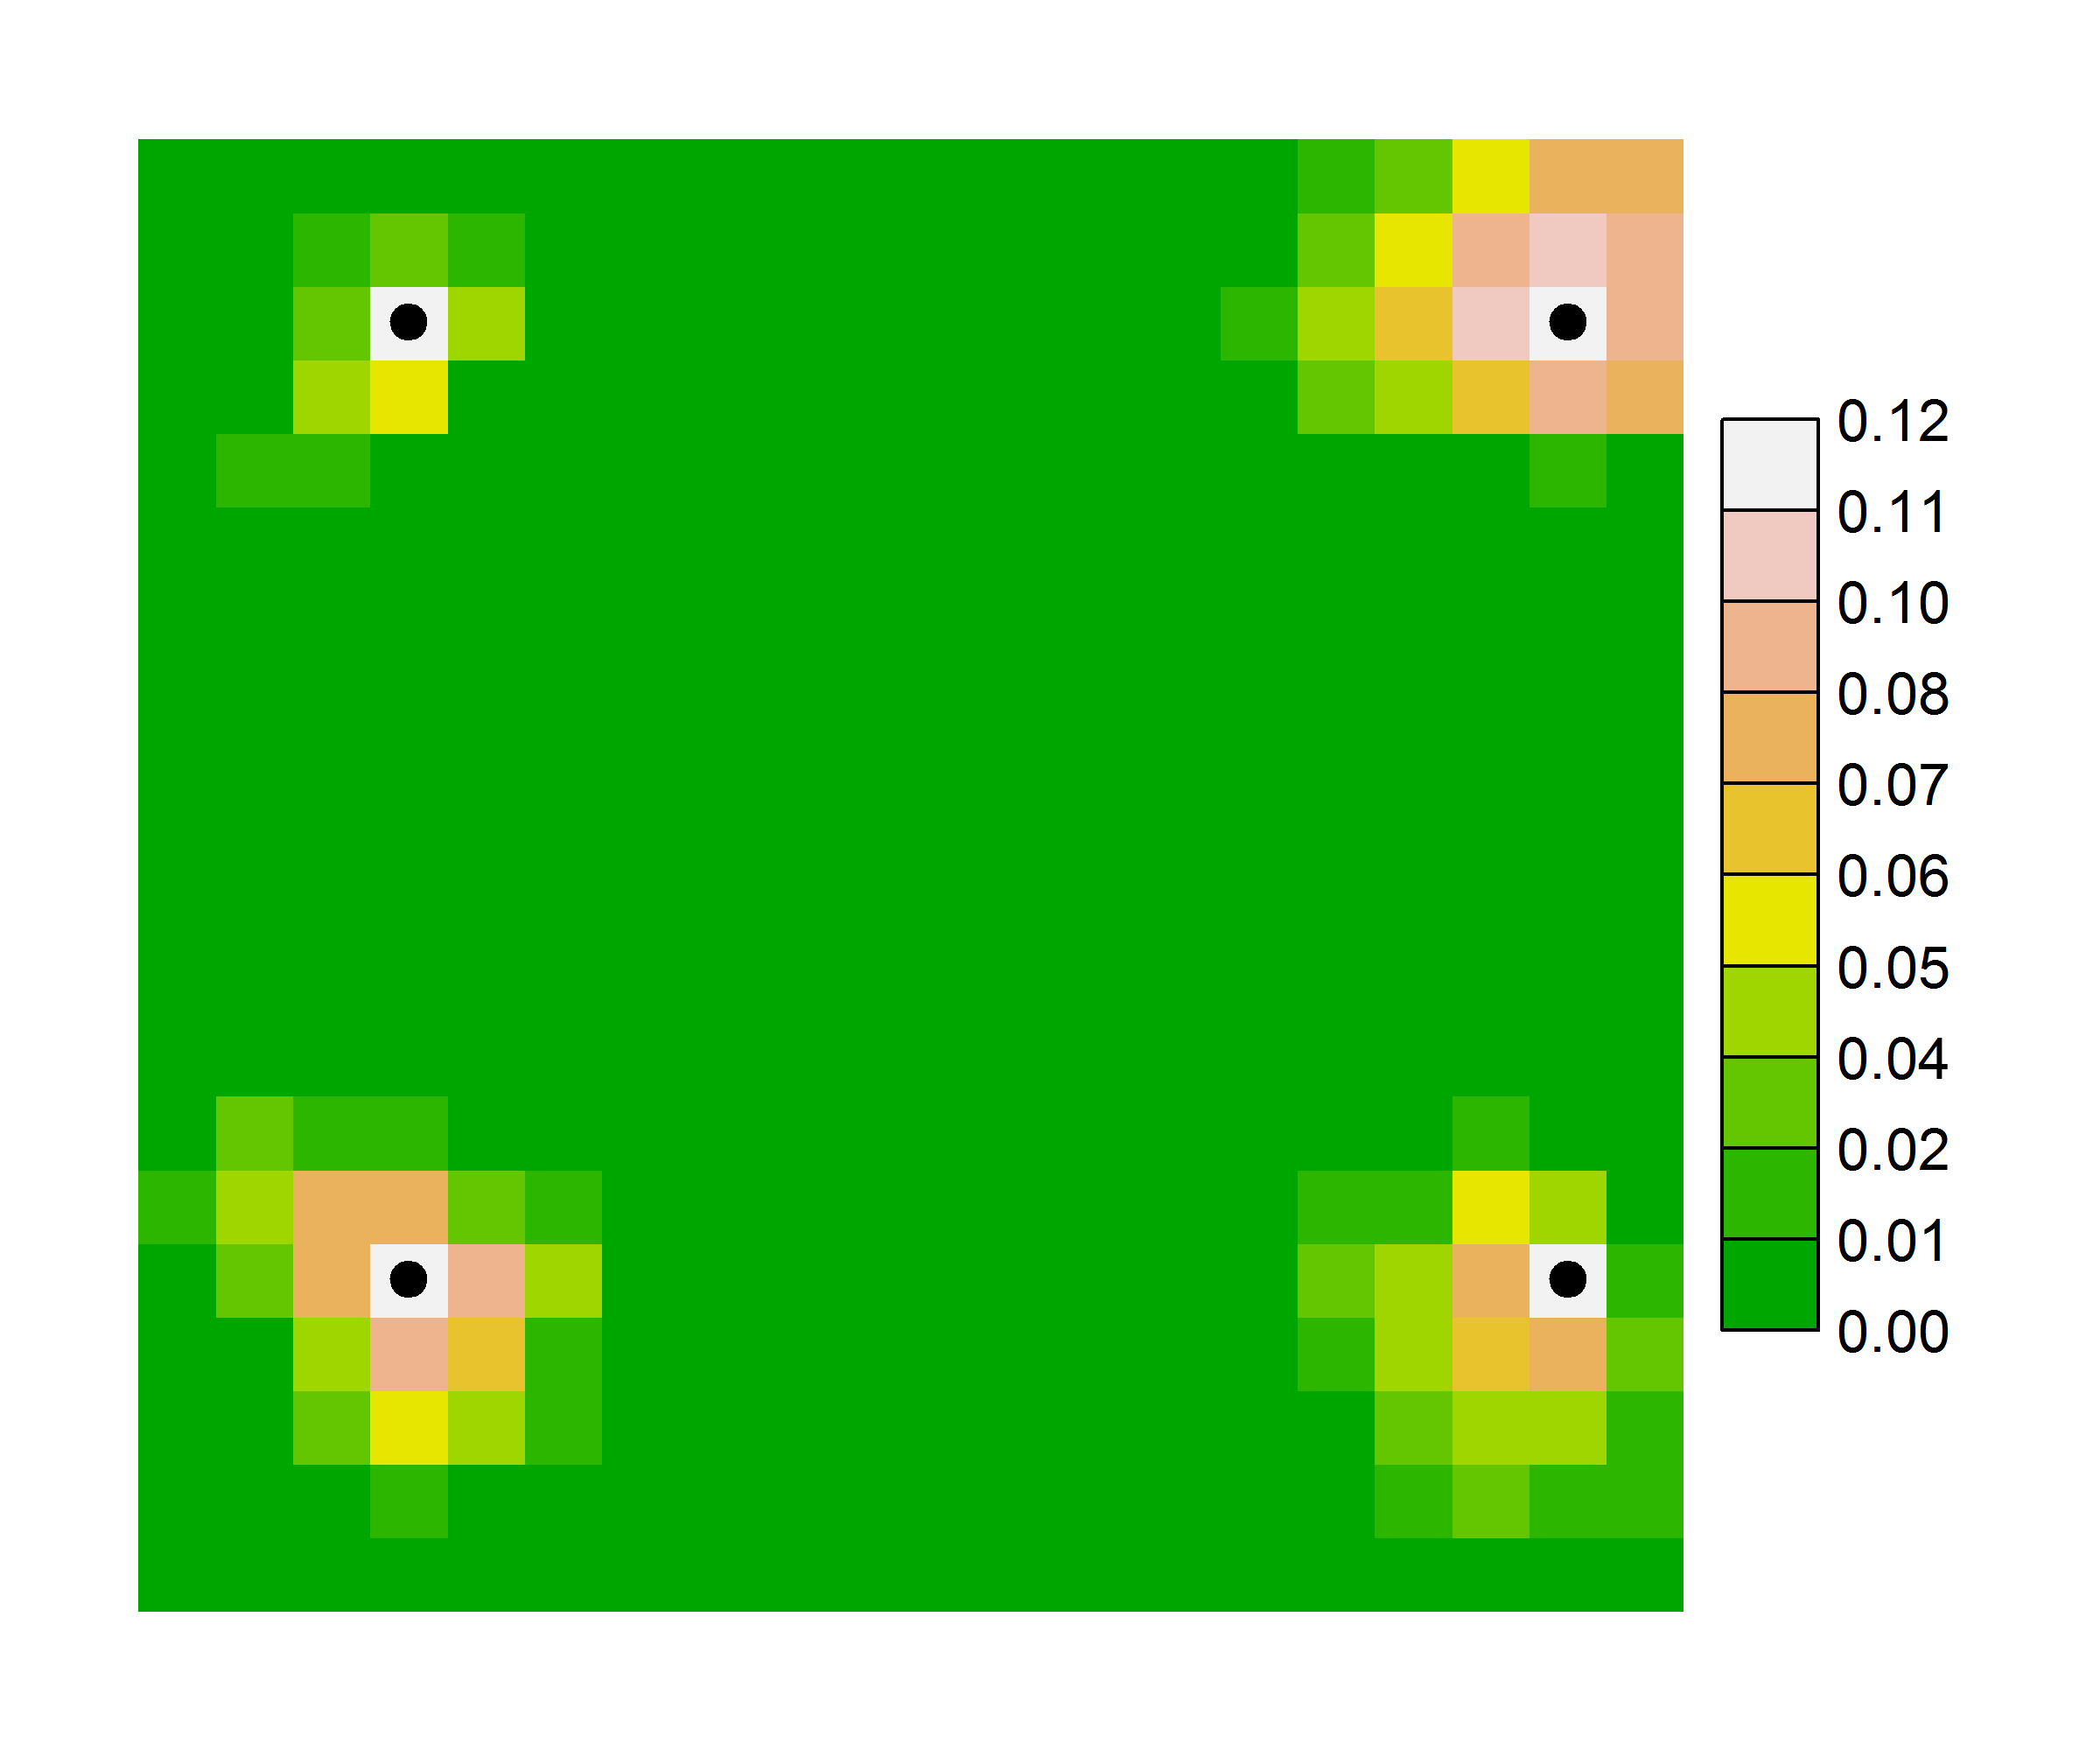
\includegraphics[height=5in,width=6in]{figs/home_rangesv2}
\end{center}
\caption{
Typical home ranges for 6 individuals based on the ``patchy'' cost surface.
The black dot indicates the home
  range center and the pixels around each home range center are shaded
according to the probability of encounter, if a trap were located in
that pixel.
}
\label{fig.homeranges}
\end{figure}

\clearpage
\newpage


\begin{figure}
\begin{tabular}{cc}
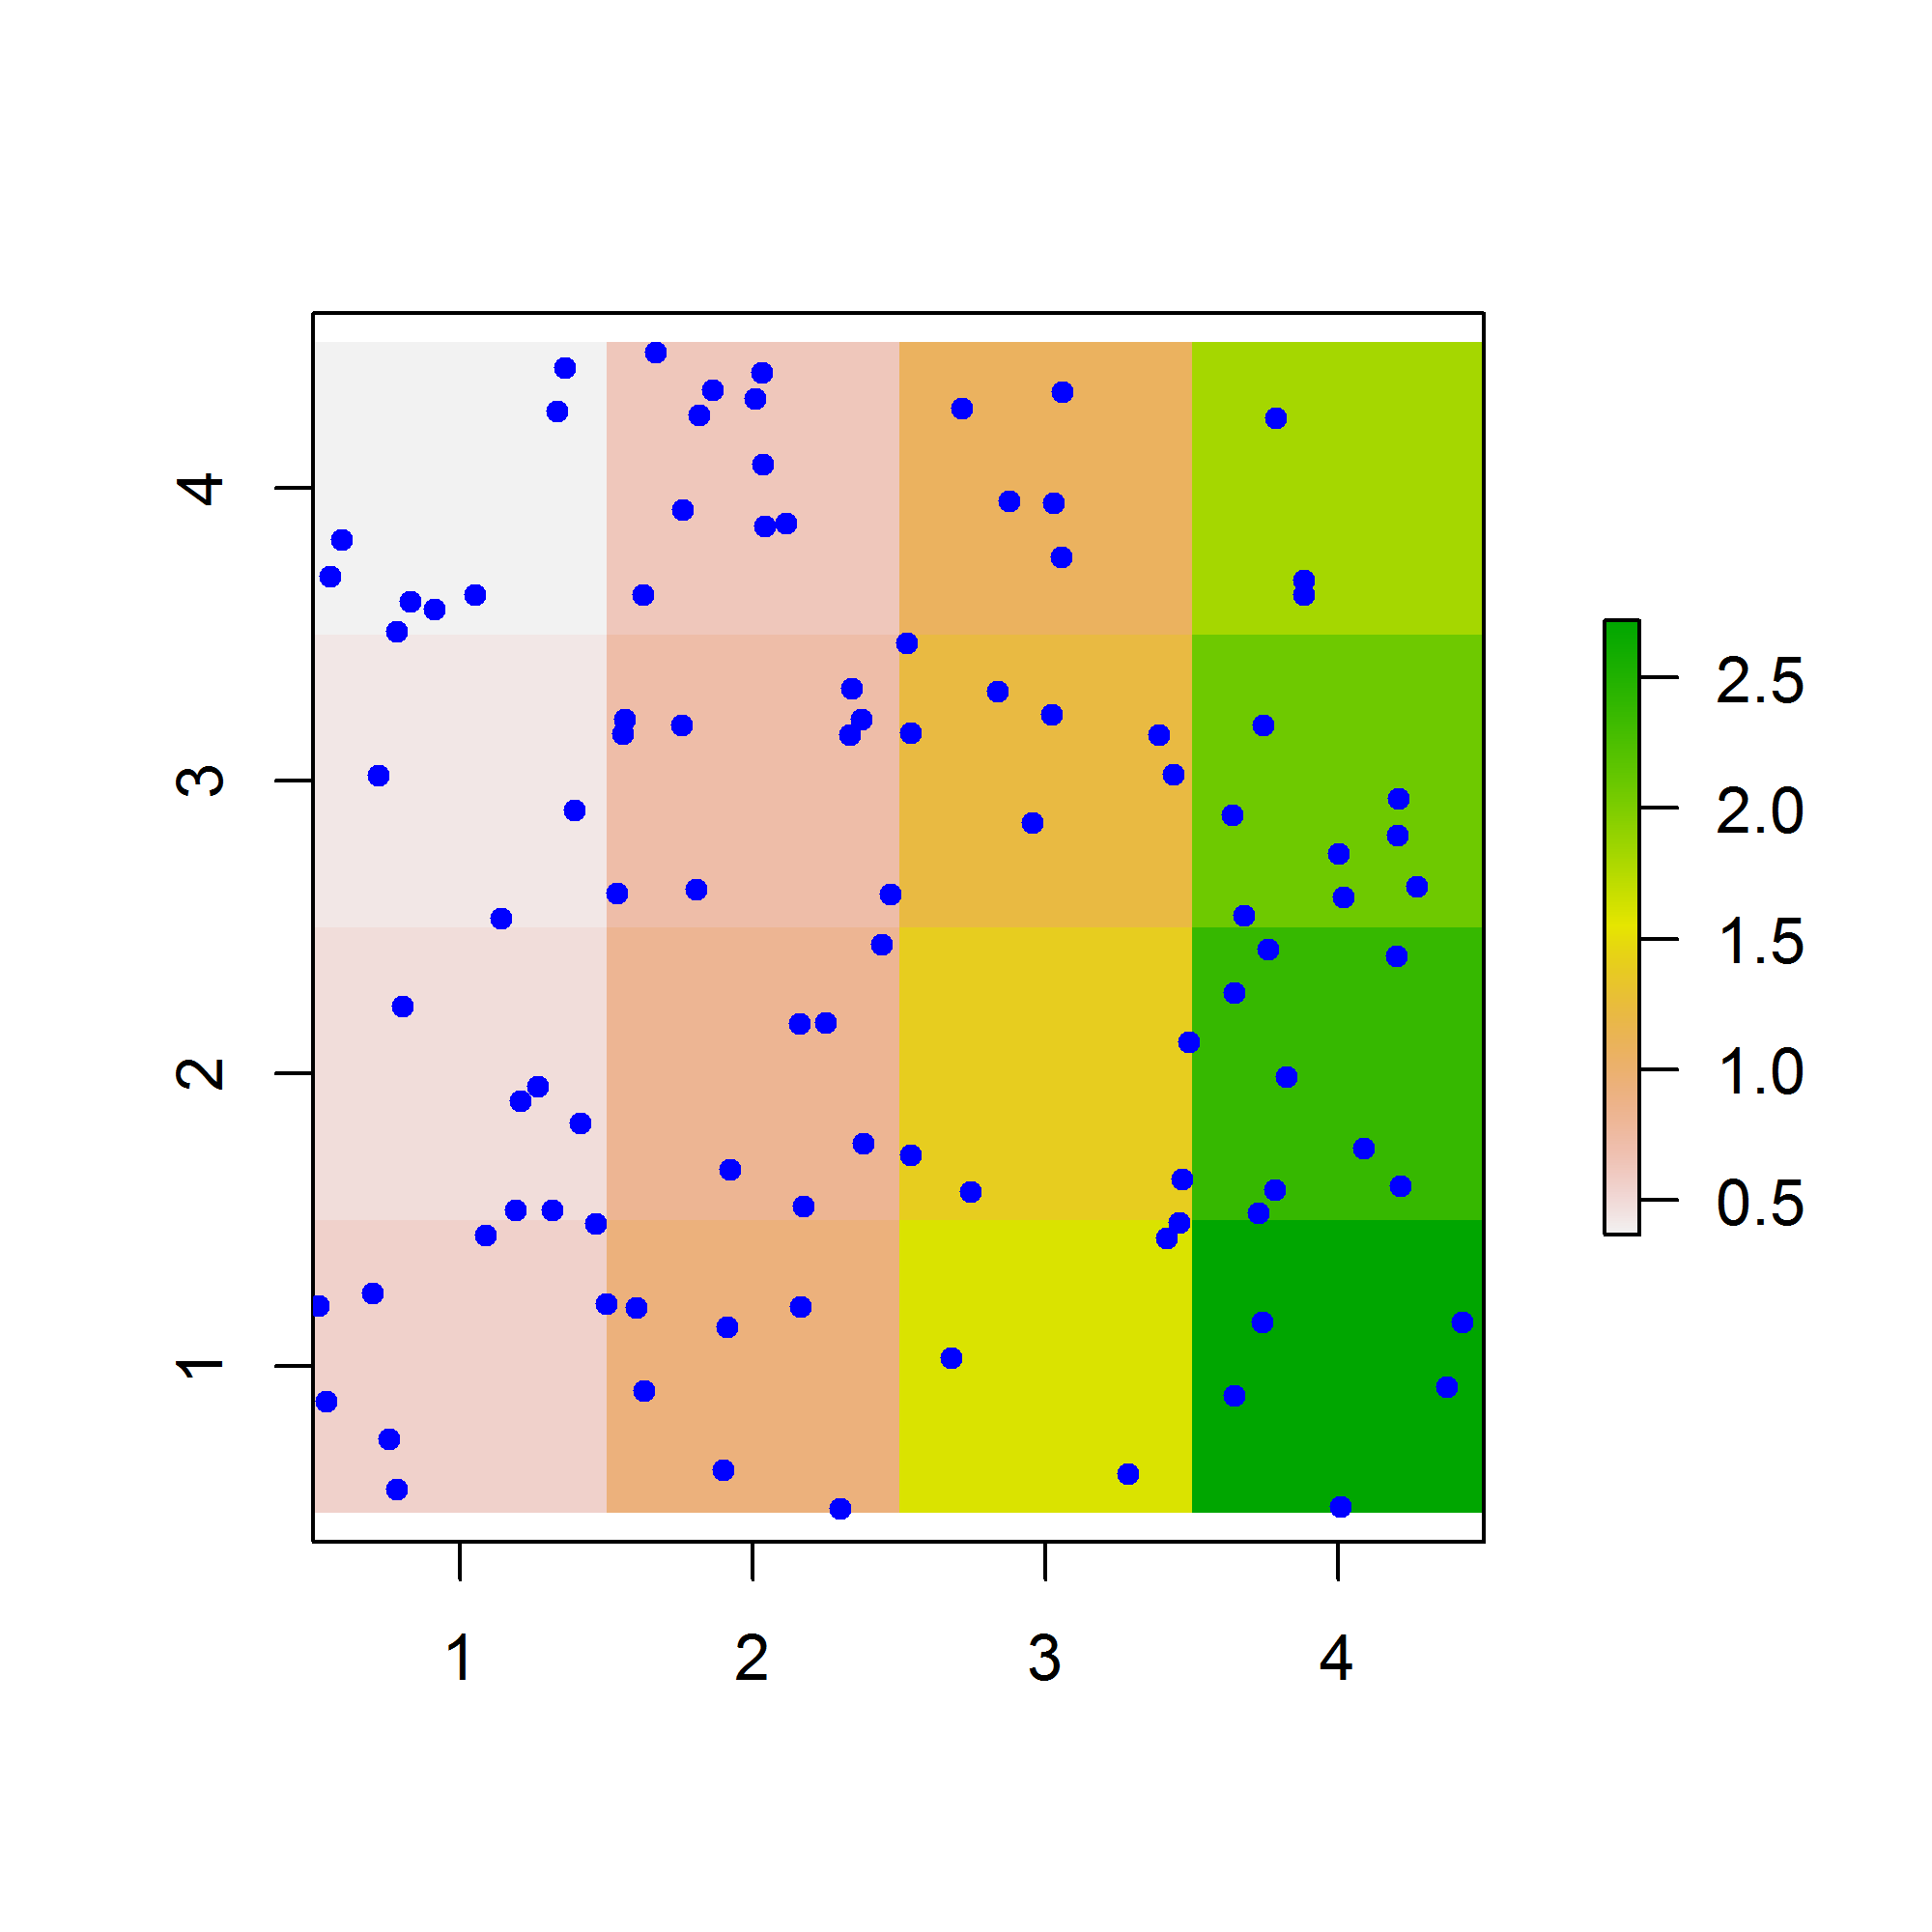
\includegraphics[height=3.25in,width=3.25in]{figs/raster_withN100}
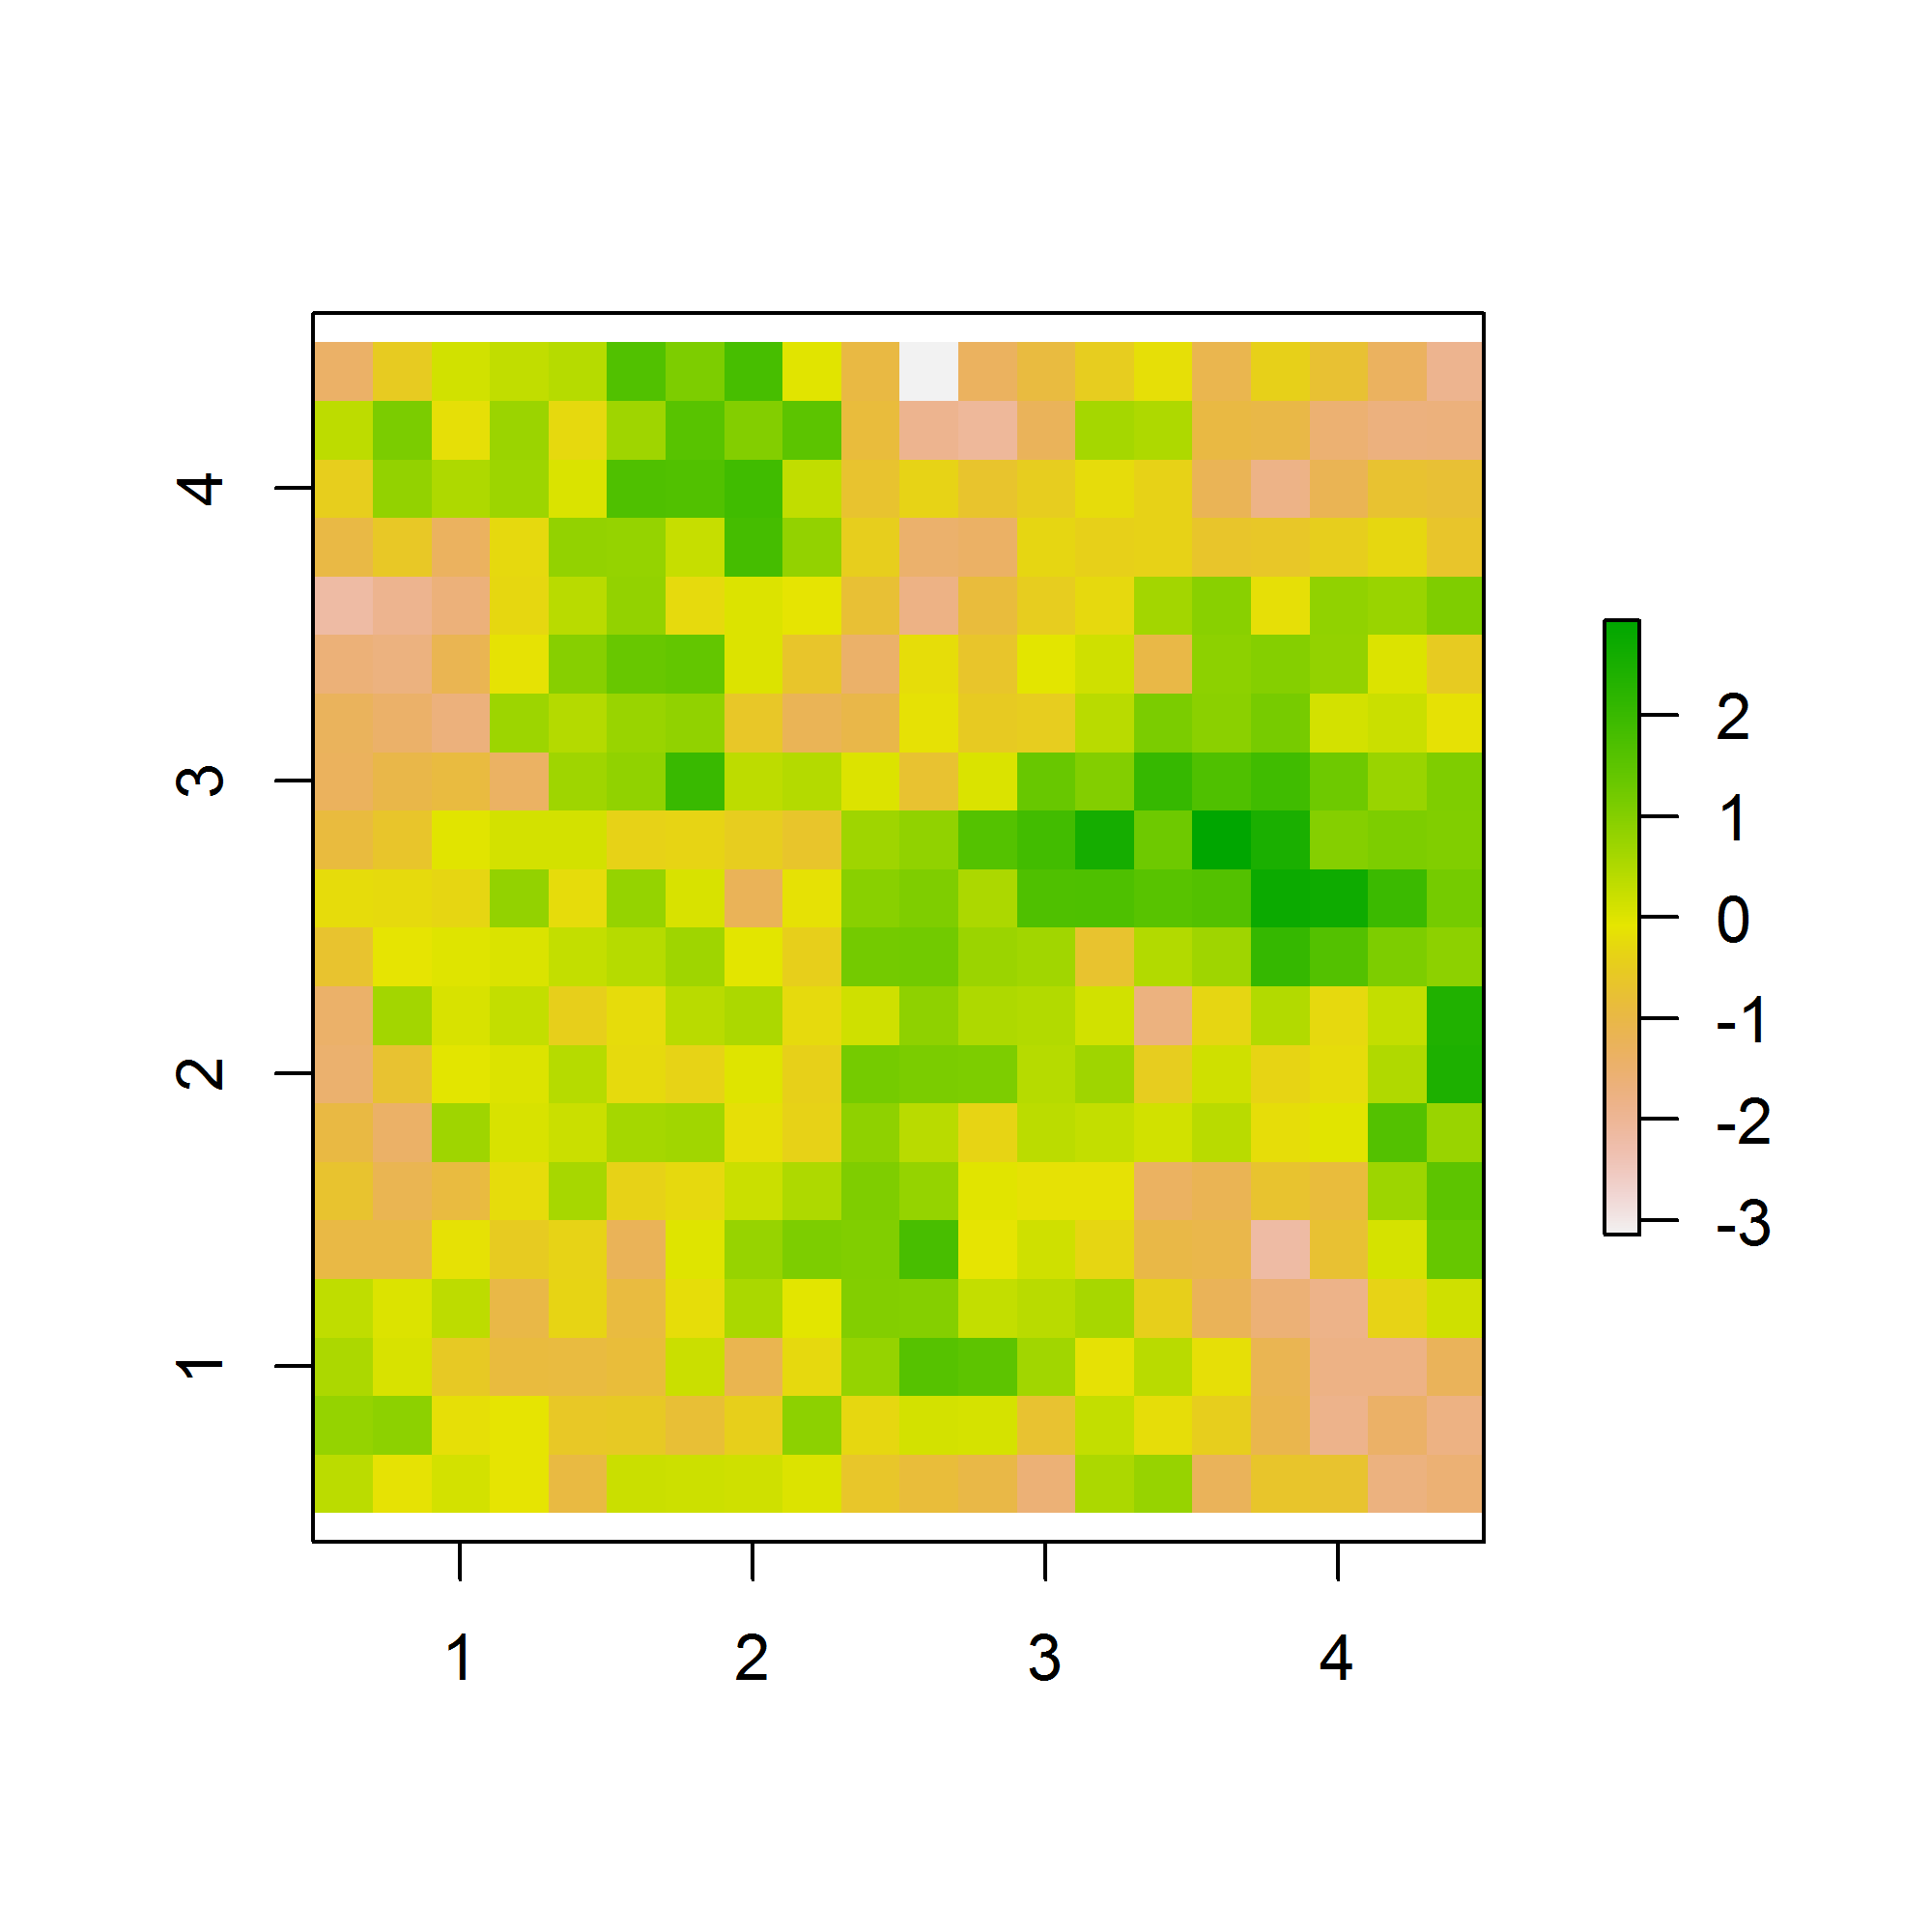
\includegraphics[height=3.25in,width=3.25in]{figs/raster_krige} &
\end{tabular}
\caption{
Two landscape covariates used for simulations. A hypothetical
  realization of $N=100$ activity centers is superimposed on the left,
along with 16 trap locations.
}
\label{ecoldist.fig.raster100}
\end{figure}


\end{comment}

\clearpage

\newpage




\end{document}






